\documentclass{scrartcl}

\usepackage[T1]{fontenc}
\usepackage[utf8]{inputenc}

\title{Mobile Dev Week 1 Lab}
\author{Daniel Coady (102084174)}
\date{16/08/2019}

\usepackage{graphicx}

\begin{document}


\maketitle

\section*{Trello Mobile vs Web}
Trello is a very popular and common tool used in task management. It features a boards system that allows
you to contain lists of cards on a project by project basis. Along with the core functionality it offers,
Trello offers both a web interface and a mobile application on both Android and iOS platforms.

\subsection*{Web Application}
\begin{figure}[h]
    \centering
    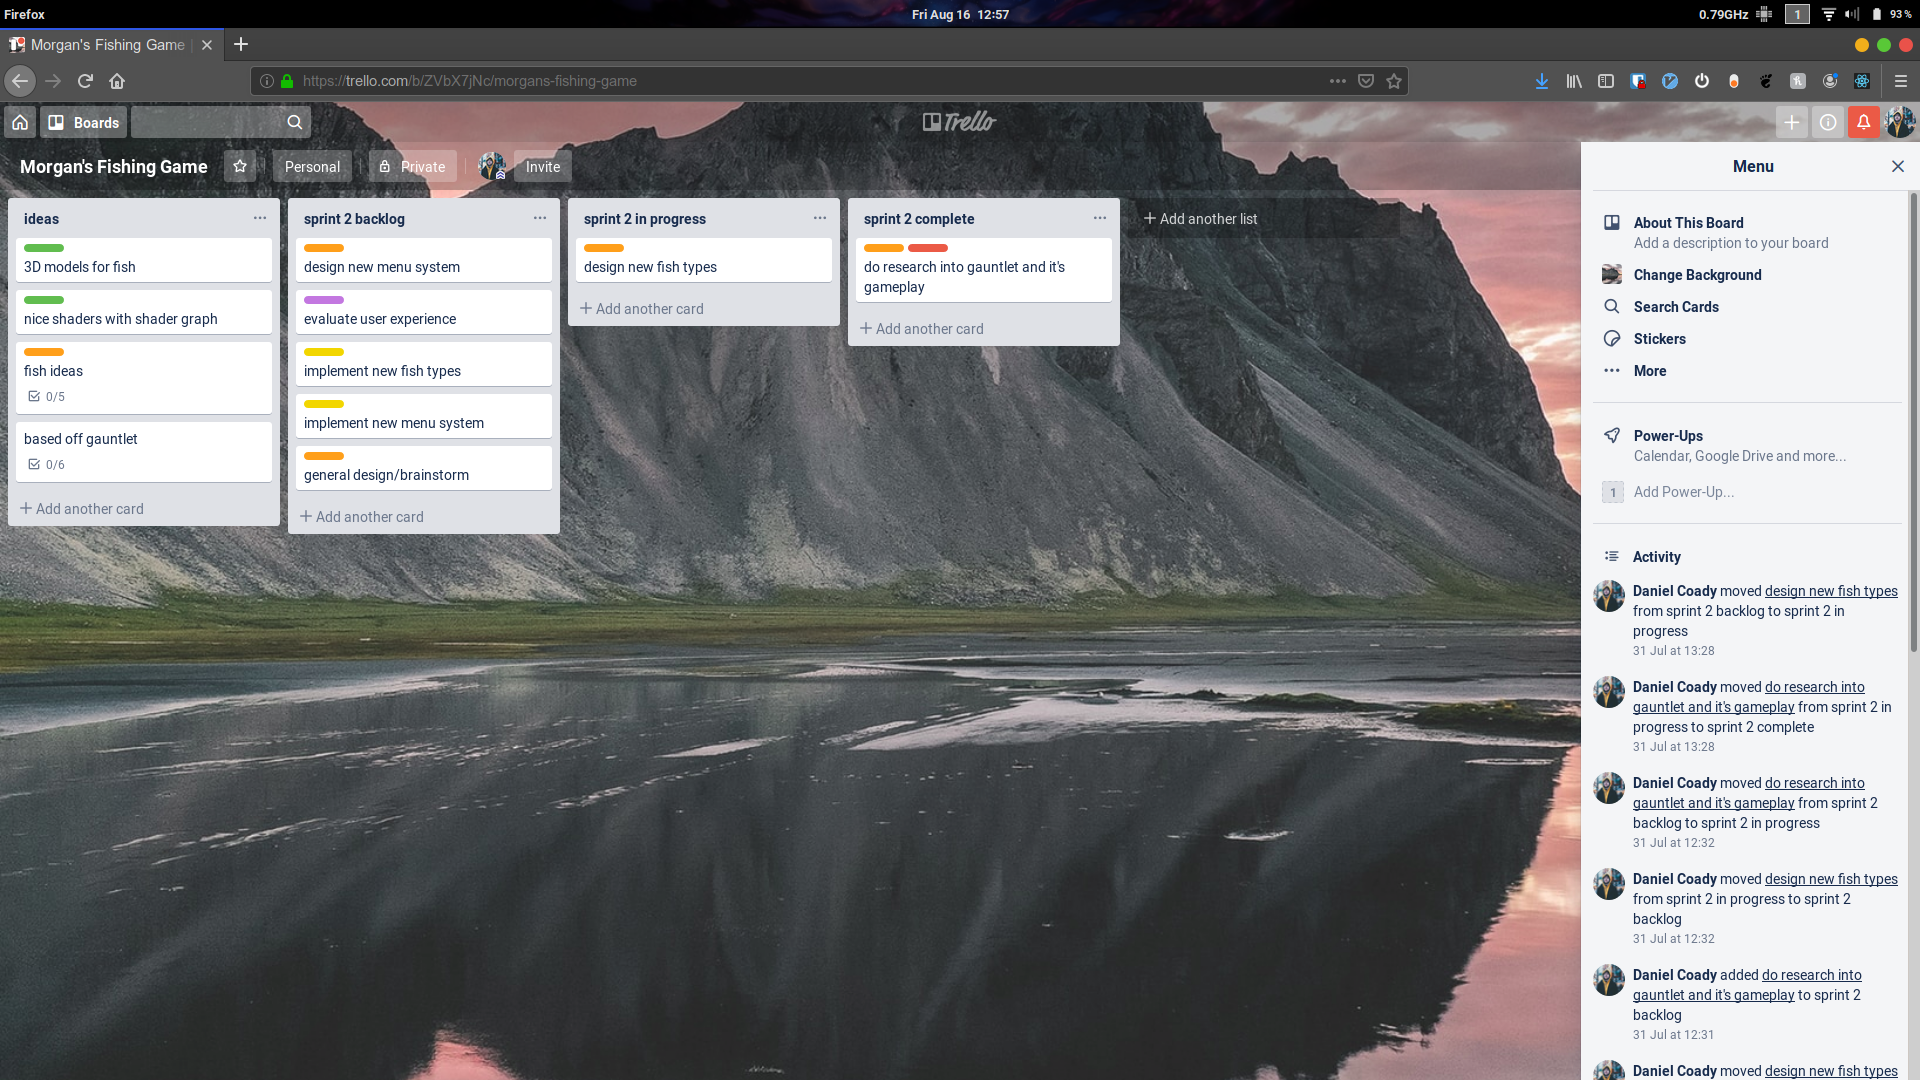
\includegraphics[scale=0.2]{images/trelloweb.png}
    \caption{The web interface for Trello}
\end{figure}

The web interface for a board is very simple and clean, dedicating most of your screen space to the lists
and cards themselves. Each list contains a set of cards and a button to add another card, and when a card
is clicked you are taken to the information about that card where extra details and edit options can be
accessed. Across the right hand side there is a menu for the board where you can change settings related
to the board and view a history of changes that have been made.

\subsection*{Mobile Application}
\begin{figure}[h]
    \centering
    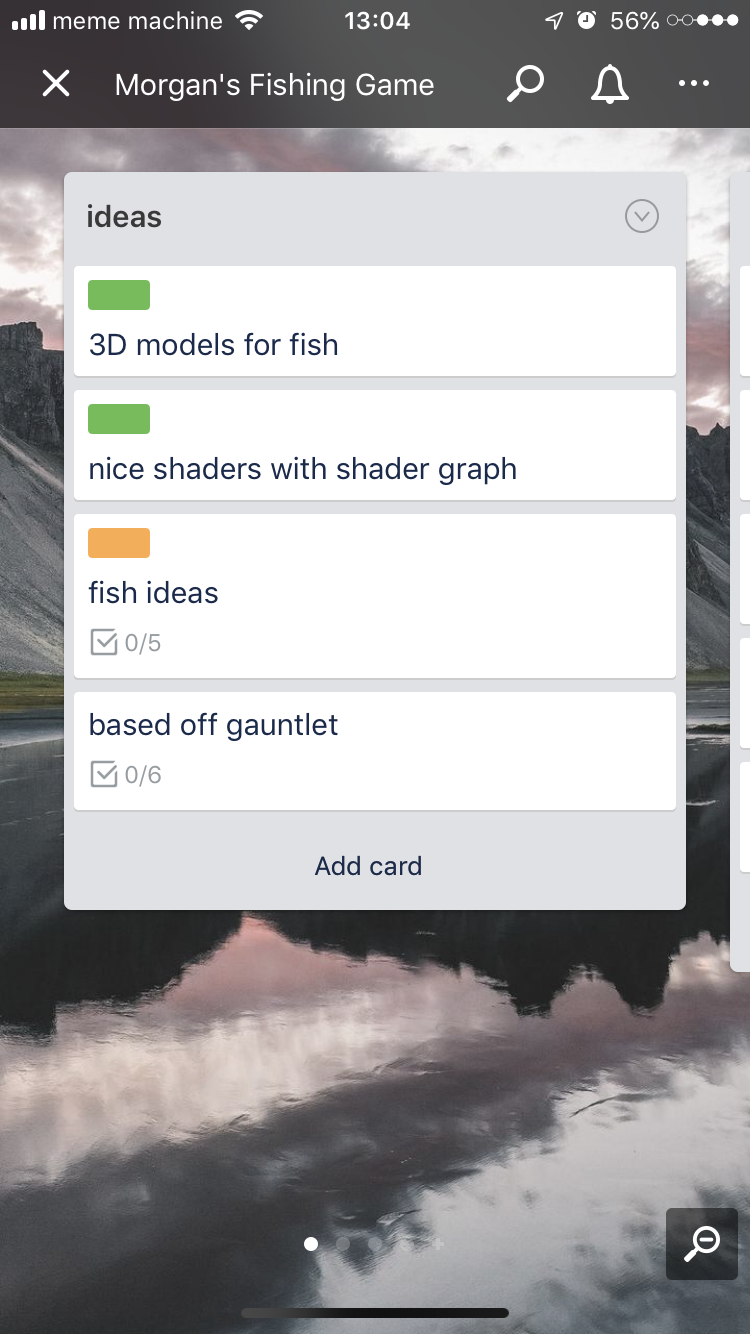
\includegraphics[scale=0.2]{images/trellomobile.png}
    \caption{The mobile (iOS) interface for Trello}
\end{figure}

Since there is very little space compared to a computer screen, the Trello mobile app has to adapt to
remain usable and accessible for it's users. On the view for a board you can see a single list at a
time and all of the cards that are within this list with the same add card button at the bottom of
each list. When you tap on a card in a list you are able to look at the information of that card just
like in the web interface, showing you extra details and edit options related to that card. Because
there is only one list viewable at a time from mobile, you have to swipe left and right to view any
additional lists that you may have on your board. Also hidden on mobile is the board menu that would
previously be on the right hand side of the screen at all times on the web interface. To access this
menu now, you must reveal it with the elipses button at the top right hand corner of the screen.

\pagebreak

\subsection*{The Key Differences}
Now that we know what both of these interfaces look like, how do they differ? of course, because we
are working with two very different screen sizes we are faced with the issue of how to fit the same
application with the same functionality onto two vastly different platforms. The way that Trello has
approached this is through hiding away anything that you don't need constant access to on mobile so
that when you are traversing the app the most useful things are always instantly at your fingertips.
The web interface on the other hand can afford to use more of the screen real estate for slightly
less important features of the application that you would still want access to. As a result of this,
both interfaces end up having a very different feel for the exact same application. The web interface
is very spacious and liberal with the different panels and menus that it shows you, while the mobile
interface wastes no space and keeps what is most important front and center as you operate the app.

\end{document}
